%Antwort auf einen Delta-Impuls.
%Die Lösung von Matlab ist zwar die gleiche, aber in einer anderen Darstellung. Sollte Matlab einen zu langen Ausdruck ausgeben, kann der Befehl simplify(ans) verwendet werden, um den Ausdruck zu vereinfachen.

\subsection{Parametrische Darstellung} %NICHT SICHER
Die parametrische Darstellung der Gewichtsfunktion $g(t)$ erhält man, indem man die Laplace-Rücktransformierte der Übertragungsfunktion bildet. Das macht man in Matlab durch folgende Befehle:\\
%syms s -> G(s)=bspw. 3*s/(1+9*s + 20*s^2) -> ilaplace(G(s)) -> t=[0;0.1;10] -> plot(t, Antwort der parametrischen Darstellung) (Da t ein Vektor ist, muss man beim Multiplizieren das Punktprodukt (Hadamad-Produkt) .* verwenden) (Alternativ kann man das mit dem fplot befehl machen, da spart man sich das Hadamad-Produkt) -> xlabel (Mit den Befehlen xlabel und ylabel kann man die Achsen beschriften) -> ylabel Gewichtsfunktion
\hspace*{0.5cm}\texttt{syms s t}\\
\hspace*{0.5cm}\texttt{G(s)=-25/(10*s+1)}\\
\hspace*{0.5cm}\texttt{g(t)=ilaplace(G(s))}\\
Alternativ lässt sich die Gewichtsfunktion auch durch Ableiten der Übertragungsfunktion $h(t)$ berechnen. In Matlab lässt sich das durch den Befehl \texttt{g(t) = diff(h(t))} bewerkstelligen.\\\\
In beiden Fällen liefert Matlab das Ergebnis:
\begin{equation*}
    g(t)=-\frac{5*e^{\frac{-t}{10}}}{2}
\end{equation*}

\subsection{Nichtparametrische Darstellung}
\subsubsection{Plot mit Matlab}
Nach der Berechnung der Gewichtsfunktion $g(t)$ lässt sich diese durch folgende Befehle in Matlab plotten:
\texttt{t=[0:1:100]}\\
\texttt{t, g(t)}\\
Das von Matlab gelieferte Ergebnis ist in der folgenden Abbildung dargestellt:
\begin{figure}[H]
    \centering
    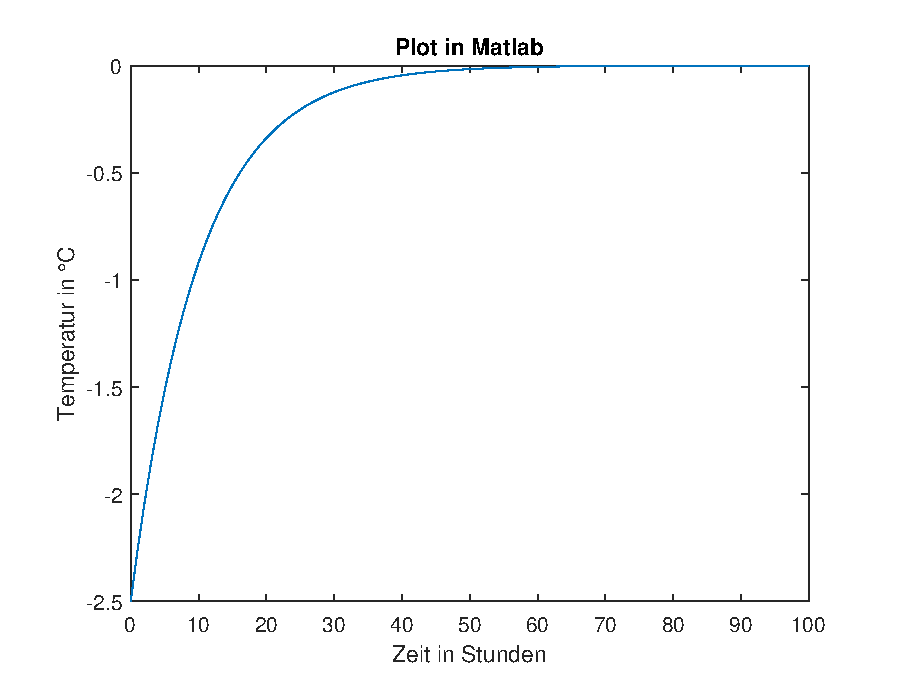
\includegraphics[width=10cm]{images_2/Gewichtsfunktion/gewichtsfkt_plot_mit_matlab.eps}
    \caption{Impulsantwort: Plot in Matlab}
\end{figure}

\subsubsection{Plot mit Step-Funktion}
Den selben Plot erhält man in Matlab auch über die \texttt{impulse}-Funktion. Diese lässt sich durch folgende Befehle anzeigen:\\
\hspace*{0.5cm}\texttt{sys = tf([-25],[10 1])}\\
\hspace*{0.5cm}\texttt{impulse(sys)}\\
Das von Matlab gelieferte Ergebnis ist in der folgenden Abbildung dargestellt.
\begin{figure}[H]
    \centering
    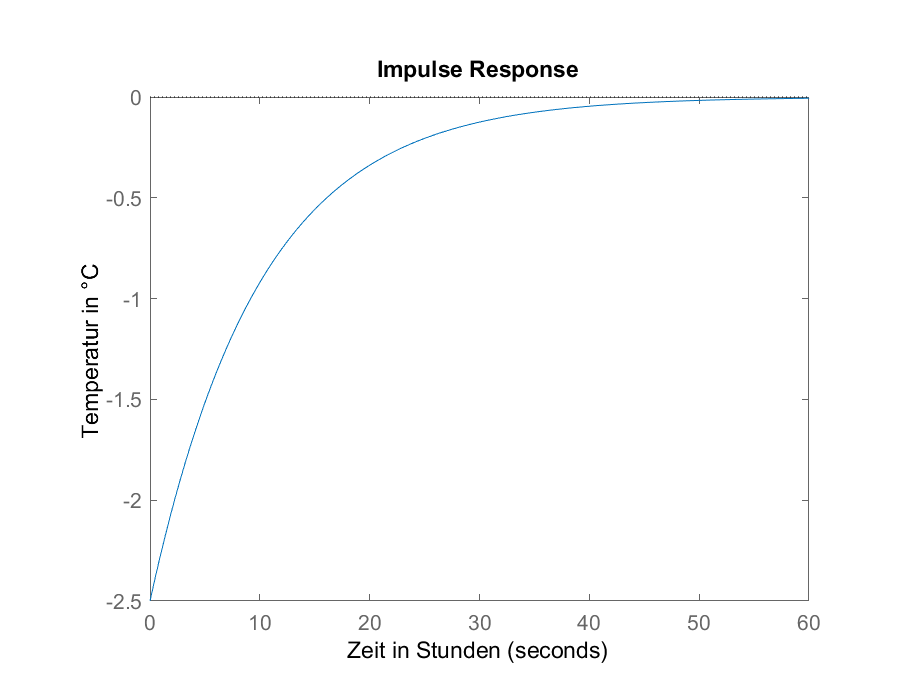
\includegraphics[width=10cm]{images_2/Gewichtsfunktion/gewichtsfkt_impulse.eps}
    \caption{Impulsantwort: Plot mit \texttt{impulse}-Funktion}
\end{figure}

\subsubsection{Plot mit Simulink}
Das Ergebnis eines Deltaimpulses kann in Simulink simuliert werden, indem die Übertragungsfunktion mit $s$ multipliziert wird. Die Simulink-Schaltung und der dazu gehörige Plot sehen wie folgt aus:
\begin{figure}[H]
    \centering
    \includegraphics[width=12cm]{images_2/Gewichtsfunktion/impuls_simulink_schaltung.png}
    \caption{Impulsantwort: Simulink-Schaltung}
\end{figure}
\begin{figure}[H]
    \centering
    \includegraphics[width=10cm]{images_2/Gewichtsfunktion/impulsantwort_simulink.png}
    \caption{Impulsantwort: Plot mit Simulink}
\end{figure}
